\documentclass[11pt]{beamer}
\usetheme{Warsaw}
\usepackage[utf8]{inputenc}
\usepackage{amsmath}
\usepackage{amsfonts}
\usepackage{amssymb}
\usepackage{color}
\usepackage{siunitx}


\usepackage{tikz}
\usetikzlibrary{shapes,snakes,arrows,positioning}
\usetikzlibrary{%
	calc,%
	decorations.pathmorphing,%
	fadings,%
	shadings%
}

% Define box and box title style
\tikzstyle{mybox} = [draw=red, fill=blue!20, very thick,
    rectangle, rounded corners, inner sep=10pt, inner ysep=20pt]
\tikzstyle{fancytitle} =[fill=red, text=white]

\author{Arindam Basu}
\title{Leak Detection}
%\setbeamercovered{transparent} 
%\setbeamertemplate{navigation symbols}{} 
%\logo{} 
%\institute{} 
%\date{} 
%\subject{} 
\begin{document}

\begin{frame}
\titlepage
\end{frame}

%\begin{frame}
%\tableofcontents
%\end{frame}


\begin{frame}
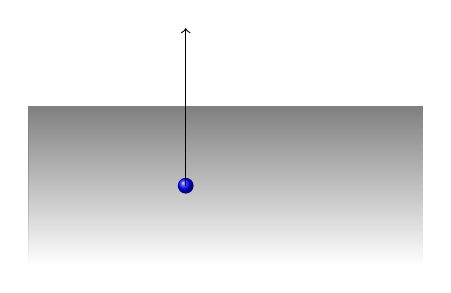
\begin{tikzpicture}
  \draw[gray,fill=gray,path fading=south] (0,0) rectangle +(5,-2);% sample
  \shade[ball color=blue] (2,-1) circle (.1cm);
  \draw[->] (2,-1)--(2,1);
  
\end{tikzpicture}
\end{frame}


\begin{frame}{• Vacuum Leaks}
\textbf{Ideal Vacuum Chamber } is chracterized by :\\
\begin{itemize}
\item Stable wall surfaces.
\item NO leaks.
\item only source of gas is the gas delivery system for process in the chamber.
\end{itemize}
In a REAL vacuum system, there can be other sources of gas besides the gas delivery system.
What problems can these other gas sources cause?
\begin{itemize}
\item It significantly increase the pump down time.
\item It contaminants in the system.
\end{itemize}



\end{frame}



\begin{frame}{• Vacuum Leaks}

\begin{itemize}
\item Loading the \textcolor{red}{ unwanted gasses} to the vacuum system and then pressure increasing in the system is known as \textbf{leak}.
\item Leak is a big problem in vacuum techniques and leak detection is a big challenge .
\item In practice there are two main aspect of leak detection:
    \begin{enumerate}
       \item  Testing the components.
	   \item Testing completed systems.
    \end{enumerate}

\item There are two kinds of leak in the vacuum system \\
\textbf{Real leak:} When the gasses passes from atmosphere into the vacuum system.\\
\textbf{Virtual leak:} When the gasses or vapors are added into the system by 
	(a) Desorption the gasses from chamber`s  wall and components
	(b) Trapped spaces




\end{itemize}


\end{frame}

\begin{frame}{Sources of gas in Vacuum System}
There are mainly three ways through which undesired gasses can get into a vacuum system and can make the pressure increases in the vacuum system.
\begin{itemize}
\item Leaks( Virtual leak and Real leak).
\item Outgassing.
\item Backstreaming
\end{itemize}

\begin{center}
\includegraphics[scale=0.4]{leaksources.jpg}
\end{center}




\end{frame}



\begin{frame}{Gas Sources-Real Leak}
A crack or hole in the vacuum system drawing molecules from the surrounding atmosphere into the work chamber.\\
Main reasons for real leak in a vacuum system are:
\begin{itemize}
\item Dirty/worn/damaged/improperly-seated seals (90 \% + cases).
\item Cracked or porous welds.
\item Loose components such as feed-throughs.
\item The migration of gas through the wall material  or O-ring
\end{itemize}

\end{frame}

\begin{frame}{Gas Sources-Virtual Leak}
Virtual leaks are caused by release of  gas trapped inside the system.
Main reasons for virtual leak in a vacuum system are:
\begin{itemize}
\item Improper welding/External Welding.
\item Screws,threads and Sleeves.
\item Flange Connection , O rings , particularly improper use of double O ring.
\end{itemize}

\textbf{How virtual leaks in a vacuum system can be elliminated?}
\begin{itemize}
\item Internal Welding.If internal welding is not possible then welding must be full penetration welding.
\item Screws,threads and Sleeves used in the vacuum system must be vented.
\item  Improper use of  gaskets , connections and O rings , particularly double O ring.
\end{itemize}


\end{frame}










\begin{frame}{Gas Sources-Back Streaming}
\begin{itemize}
\item An ideal pump only removes molecules from the vacuum system and does not add any molecule in the system.
\item In reality some of the vacuum pumps introduce molecule in the vacuum system.
\item Oil from diffusion pumps and rotary vane pumps are main reason for oil backstreaming in the system.
\item Oil-based pumping systems are designed with anti-suckback valves, and cold traps to minimize backstreaming.
\item Oil Backstreaming  is the primary reason for the gradual replacement of oil-based pumps with “dry” pumps such as roots blower or diaphragm pump.
\end{itemize}


\end{frame}



\begin{frame}{Advantages and Disadvantages of Helium as the tracer gas}

\textbf{Advatages}
\begin{itemize}
\item Helium is very light and small
\item Low concentration in air (0.0005\%)
\item Permits dynamic testing
\item Permits non-destructive testing
\item Helium is safe

\end{itemize}

\textbf{Disadvatages}
\begin{itemize}
\item Helium is very costly.
\item Can be a source of permeation if a lot a glass item is present.

\end{itemize}
\end{frame}




\begin{frame}{Vacuum Leak- Summary}
\begin{itemize}
\item Has the pressure in the system changes since yesterday?
\item Can any section of the vacuum system be isolated?
\item Has the gauge calibration been checked?
\item Are there any sources of vapors present in the system?
\item Has a real leak been established even though not found?
\item Can the leak,that has been established, be tolerated at least for some time?
\item Have any different type of cleaning material is used after the last exposure to the atmosphere?
\item Is anything added or modified in the interior of the vacuum system?
\item Is there any evidence of an air leak from an RGA spectrum with peaks corresponding to masses 14, 28, 32?
\end{itemize}


\end{frame}





\begin{frame}{• Mean Free Path-2}


MFP increases as the pressure decreases.Approx relation $ l (cm) ~= \frac{.005}{P (Torr)} $
\begin{center}
    \begin{tabular}{ | l | l | l | }
    \hline
    Pr. & Molecular Density & MFP\\ \hline
   
    1013 mbar (ATM) 
    & \num[round-precision=2,round-mode=figures,
     scientific-notation=true]{3e-19} 
    & \num[round-precision=2,round-mode=figures,
    scientific-notation=true]{6.4e-5} mm  \\ \hline
	
	\num[round-precision=2,round-mode=figures,
     scientific-notation=true]{1e-3}  mbar  
    & \num[round-precision=2,round-mode=figures,
     scientific-notation=true]{4e-13} 
    & 5.1 mm  \\ \hline
     
    \num[round-precision=2,round-mode=figures,
     scientific-notation=true]{1e-9}  mbar  
    & \num[round-precision=2,round-mode=figures,
     scientific-notation=true]{4e-7} 
    & 50 km  \\ \hline 
     
    
                   
    
    %\hline
    \end{tabular}
\end{center}	





\end{frame}



\begin{frame}{• Why Vacuum is Needed}



\begin{center}


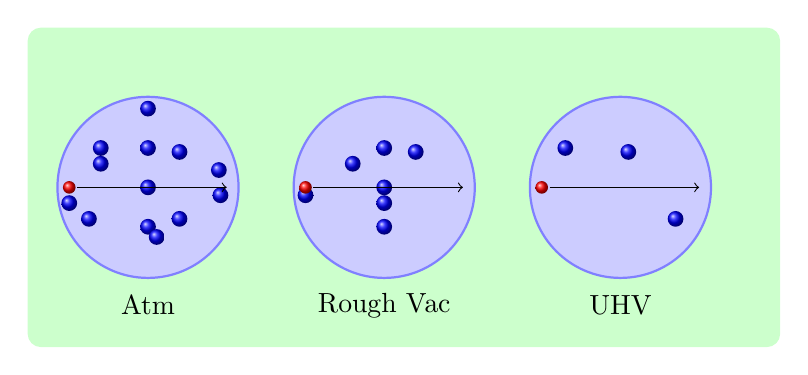
\begin{tikzpicture}[scale=1.0]
   
 \tikzstyle{vessel}=[circle,draw=blue!50,fill=blue!20,thick,
inner sep=0cm,minimum size=2.3cm]




\draw [fill=green!20,ultra thick,green!20,rounded corners] (-1.5,-2) rectangle (8,2);

\node[vessel] (V_ATM) {};
\node[vessel] (V_RV) [node distance=3cm,right of=V_ATM] {};
\node[vessel] (V_UHV) [node distance=3cm,right of=V_RV] {};

\node (ATM)[node distance=1.5cm,below of=V_ATM] {Atm};
\node (rv)[node distance=1.5cm,below of=V_RV] {Rough Vac};
\node (uhv)[node distance=1.5cm,below of=V_UHV] {UHV};

% First Vessel Molecules
\shade[ball color=blue] (0,.5) circle (.1cm);
\shade[ball color=blue] (.4,.45) circle (.1cm);
\shade[ball color=blue] (.9,.22) circle (.1cm);
\shade[ball color=blue] (-.6,.5) circle (.1cm);
\shade[ball color=blue] (-1.0,-.2) circle (.1cm);

\shade[ball color=blue] (0,-.5) circle (.1cm);
\shade[ball color=blue] (.11,-.63) circle (.1cm);
\shade[ball color=blue] (-0.75,-.4) circle (.1cm);
\shade[ball color=blue] (0,0) circle (.1cm);

\shade[ball color=blue] (-.6,.3) circle (.1cm);
\shade[ball color=blue] (.4,-.4) circle (.1cm);
\shade[ball color=blue] (0,1.0) circle (.1cm);
\shade[ball color=blue] (.92,-.1) circle (.1cm);


% Second Vessel Molecules

\shade[ball color=blue] (3,.5) circle (.1cm);

\shade[ball color=blue] (3.4,.45) circle (.1cm);

\shade[ball color=blue] (3.0,-.2) circle (.1cm);

\shade[ball color=blue] (3,-.5) circle (.1cm);

\shade[ball color=blue] (3,0) circle (.1cm);

\shade[ball color=blue] (2.6,.3) circle (.1cm);

\shade[ball color=blue] (2,-.1) circle (.1cm);




% Second Vessel Molecules

\shade[ball color=blue] (5.3,.5) circle (.1cm);

\shade[ball color=blue] (6.1,.45) circle (.1cm);




\shade[ball color=blue] (6.7,-.4) circle (.1cm);




% Beam 
\shade[ball color=red] (-1,0) circle (.08cm);

\shade[ball color=red] (2,0) circle (.08cm);

\shade[ball color=red] (5,0) circle (.08cm);
% Beam Path
\draw[->] (-0.9,0)--(1,0);

\draw[->] (2.1,0)--(4,0);

\draw[->] (5.1,0)--(7,0);

\end{tikzpicture}

\end{center}

		
To move a particle in straight line over a long distance.

\end{frame}


\begin{frame}{• Surface Phenomena}

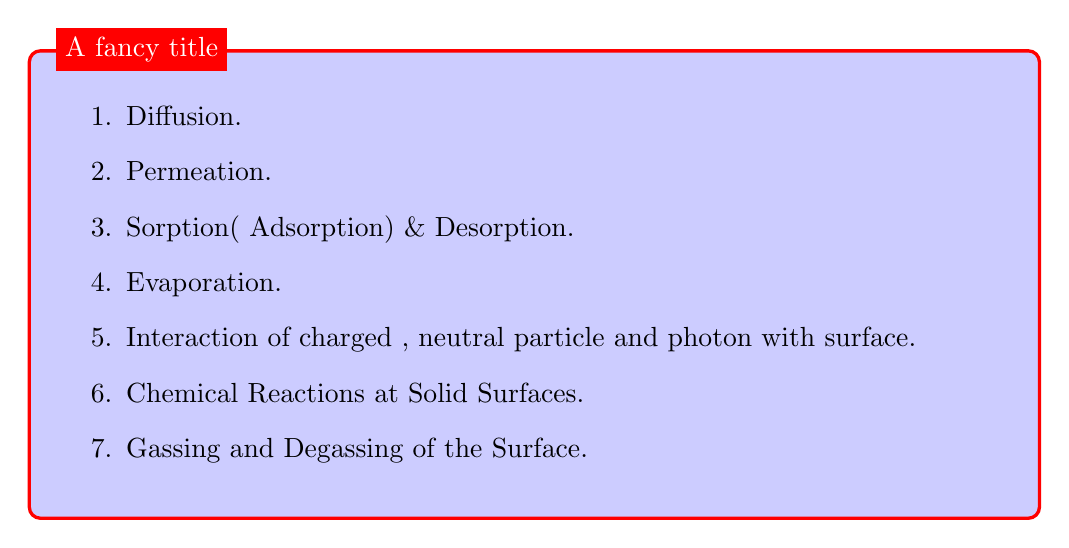
\begin{tikzpicture}
\node [mybox] (box){%
    \begin{minipage}{1.00\textwidth}
        \begin{enumerate}
			\item Diffusion.
			\item Permeation.
			\item Sorption( Adsorption) \& Desorption.
	   	 	\item Evaporation.
			\item Interaction of charged , neutral particle and photon with surface.
			\item Chemical Reactions at Solid Surfaces.
			\item Gassing and Degassing of the Surface.
	
	\end{enumerate}
    \end{minipage}
};
\node[fancytitle, right=10pt] at (box.north west) {A fancy title};
%\node[fancytitle, rounded corners] at (box.east) {$\clubsuit$};
\end{tikzpicture}%




	

		
		


\end{frame}


\begin{frame}{• Surface Phenomena(Contd. )}

\begin{enumerate}
\item DIFFUSION can occur in presence of concentration gradients in the gases dissolved in solids. Temperature dependent process.

\item PERMEATION can occur by gas transfer from the outside atmosphere through the wall into vacuum space through diffusion process. Temperature dependent process. Significant amount of helium can permeate through glass walls into vacuum.

\item SORPTION If a material traps the air molecules in its surface then the  process is called sorption.

\end{enumerate}

	


\end{frame}




\end{document}